\documentclass{ctexart}

% 浮动体
% 实现灵活分页(避免无法分割的内容产生的页面留白)
% 给图表添加标题
% 交叉引用

% figure环境(table环境与之类似)
% \begin{figure}[<允许位置>]
%   <任意内容 >
% \end{figure}

% <允许位置>参数(默认tbp)
% h,此处(here)-代码所在的上下文位置
% t,页顶(top)-代码所在页面或之后页面的顶部
% b,页底(bottom)-代码所在页面或之后页面的底部
% p,独立一页(page)-浮动页面

% 标题控制(caption、bitaption等宏包)
% 并排与子图表(subcaption、subfig、floatrow等宏包)
% 绕排(picinpar、wrapfig等宏包)
\usepackage{graphicx}
\graphicspath{{figures/},{pics/}}

\begin{document}
\LaTeX{} 中插图 系统的吉祥物---小狮子 见图\ref{fig-lion}
\begin{figure}[htbp]
    \centering
    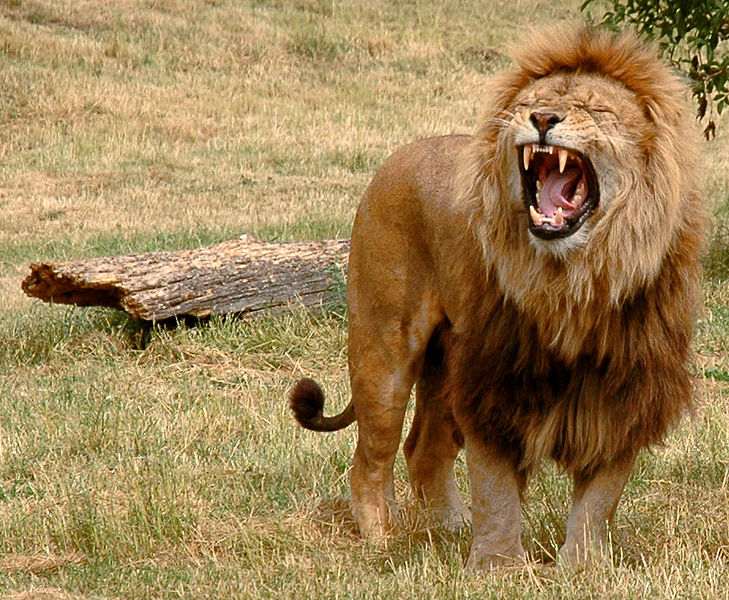
\includegraphics[scale=0.3]{lion}
    \caption{系统的吉祥物---小狮子} \label{fig-lion}
\end{figure}


在\LaTeX{}中的表格:
也可以使用表\ref{tab-score}
    \begin{table}[h]
        \centering
        \caption{考试成绩单}   \label{tab-score}
        \begin{tabular}{|l ||  c | c | c | p{1.5cm} |}
            \hline
            姓名 & 语文 & 数学 & 外语 & 备注        \\
            \hline \hline
            张三 & 97   & 100 & 93  & 优秀      \\
            \hline
            李四 & 75   & 64  & 52  & 补考另行通知  \\
            \hline
        \end{tabular}
    \end{table}


\end{document}